\chapter{Split multivariate mass fits}
\label{app:SplitMassFits}

\setcounter{actualchapter}{1}
\def\chaptertag{A}

This \lcnamecref{app:SplitMassFits} contains the figures of the multivaraite fits to partial \BsDsK~samples, introduced in \cref{sec:BsDsK_TD_MDFit_Validation}.
%
\begin{figure}[hp] \centerfloat
    \fontsize{8}{9.6}\selectfont
    \begin{subfigure}{.48\textwidth} \centerfloat
        \begin{tikzpicture}
            \node[anchor=south west,inner sep=0] (image) at (0,0) {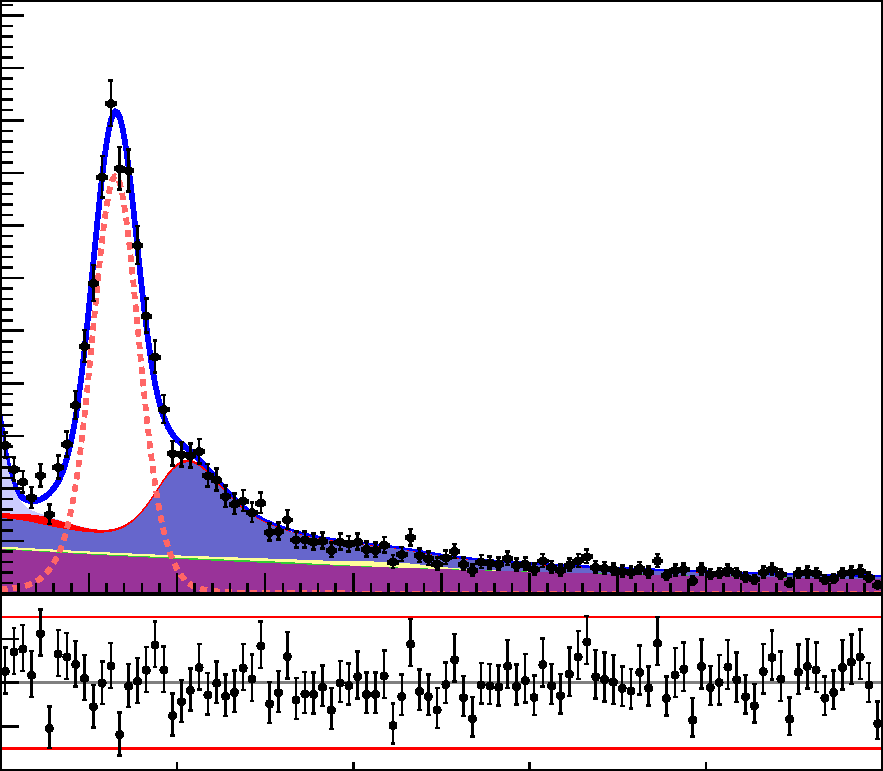
\includegraphics[width=0.675\textwidth]{appendices/mass_Bs2DsK_BeautyMass_up_all_run1_split}};
            \begin{scope}[x={(image.south east)},y={(image.north west)}]
                \foreach \x/\xtext in {5300, 5400, ..., 5800}
                {
                    \tikzmath{\xpos = (\x - 5300) / (5800 - 5300);}
                    \node at (\xpos, -0.040) {\(\xtext\)};
                }
                \foreach \y in {0, ..., 11}
                {
                    \tikzmath{\ypos = (\y / 11) * 0.749 + 0.207; \ytext = 50 * \y;}
                    \node[anchor=base east] at (0.012, \ypos) {\(\pgfmathprintnumber[fixed,precision=0,fixed zerofill=true,1000 sep={}]{\ytext}\)};
                }
                \foreach \p in {0, ..., 2}
                {
                    \tikzmath{\ypos = (\p / 2) * 0.120 + .055; \ptext = (\p - 1) * 2;}
                    \node[anchor=east] at (0.012, \ypos) {\(\scriptstyle\pgfmathprintnumber[fixed,precision=0,fixed zerofill=true]{\ptext}\)};
                }
                \node[anchor=east] at (1.0, -0.14) {\({m(\DsmpKpm)}~[\si{\MeVcc}]\)};
                \node[rotate=90,anchor=east,inner xsep=0pt,outer xsep=0pt] at (-0.20, 1.0) {\({\text{Candidates}/(\SI{5.0}{\MeVcc})}\)};
                \node[anchor=west] at (0.26, 0.92) {\large\lhcb};
            \end{scope}
        \end{tikzpicture}
        \caption{\DsmpKpm~invariant mass fit for the data taken with the \lhcb~magnet polarity up.}
    \end{subfigure}
    \begin{subfigure}{.48\textwidth} \centerfloat
        \begin{tikzpicture}
            \node[anchor=south west,inner sep=0] (image) at (0,0) {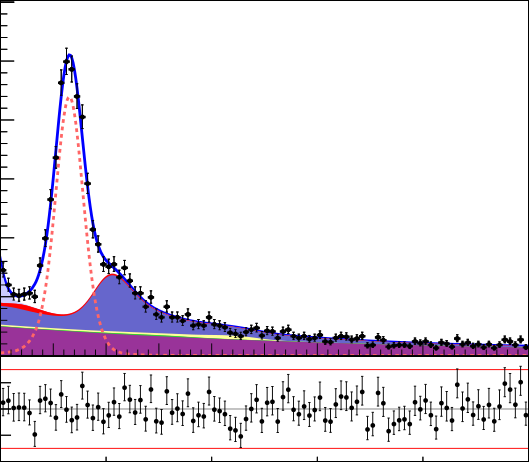
\includegraphics[width=0.675\textwidth]{appendices/mass_Bs2DsK_BeautyMass_down_all_run1_split}};
            \begin{scope}[x={(image.south east)},y={(image.north west)}]
                \foreach \x/\xtext in {5300, 5400, ..., 5800}
                {
                    \tikzmath{\xpos = (\x - 5300) / (5800 - 5300);}
                    \node at (\xpos, -0.040) {\(\xtext\)};
                }
                \foreach \y in {0, ..., 6}
                {
                    \tikzmath{\ypos = (\y / 6) * 0.760 + 0.207; \ytext = 100 * \y;}
                    \node[anchor=base east] at (0.012, \ypos) {\(\pgfmathprintnumber[fixed,precision=0,fixed zerofill=true,1000 sep={}]{\ytext}\)};
                }
                \foreach \p in {0, ..., 2}
                {
                    \tikzmath{\ypos = (\p / 2) * 0.120 + .055; \ptext = (\p - 1) * 2;}
                    \node[anchor=east] at (0.012, \ypos) {\(\scriptstyle\pgfmathprintnumber[fixed,precision=0,fixed zerofill=true]{\ptext}\)};
                }
                \node[anchor=east] at (1.0, -0.14) {\({m(\DsmpKpm)}~[\si{\MeVcc}]\)};
                \node[rotate=90,anchor=east,inner xsep=0pt,outer xsep=0pt] at (-0.20, 1.0) {\({\text{Candidates}/(\SI{5.0}{\MeVcc})}\)};
                \node[anchor=west] at (0.26, 0.92) {\large\lhcb};
            \end{scope}
        \end{tikzpicture}
        \caption{\DsmpKpm~invariant mass fit for the data taken with the \lhcb~magnet polarity down.}
    \end{subfigure}
    \\
    \begin{subfigure}{.48\textwidth} \centerfloat
        \begin{tikzpicture}
            \node[anchor=south west,inner sep=0] (image) at (0,0) {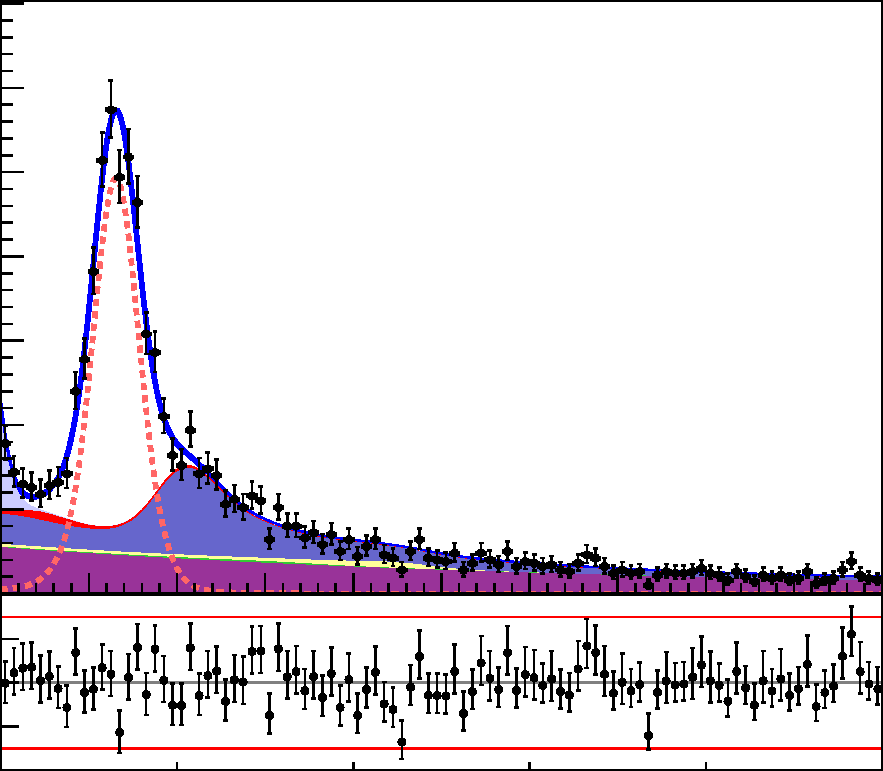
\includegraphics[width=0.675\textwidth]{appendices/mass_Bs2DsK_BeautyMass_both_all_2011_split}};
            \begin{scope}[x={(image.south east)},y={(image.north west)}]
                \foreach \x/\xtext in {5300, 5400, ..., 5800}
                {
                    \tikzmath{\xpos = (\x - 5300) / (5800 - 5300);}
                    \node at (\xpos, -0.040) {\(\xtext\)};
                }
                \foreach \y in {0, ..., 7}
                {
                    \tikzmath{\ypos = (\y / 7) * 0.760 + 0.207; \ytext = 50 * \y;}
                    \node[anchor=base east] at (0.012, \ypos) {\(\pgfmathprintnumber[fixed,precision=0,fixed zerofill=true,1000 sep={}]{\ytext}\)};
                }
                \foreach \p in {0, ..., 2}
                {
                    \tikzmath{\ypos = (\p / 2) * 0.120 + .055; \ptext = (\p - 1) * 2;}
                    \node[anchor=east] at (0.012, \ypos) {\(\scriptstyle\pgfmathprintnumber[fixed,precision=0,fixed zerofill=true]{\ptext}\)};
                }
                \node[anchor=east] at (1.0, -0.14) {\({m(\DsmpKpm)}~[\si{\MeVcc}]\)};
                \node[rotate=90,anchor=east,inner xsep=0pt,outer xsep=0pt] at (-0.20, 1.0) {\({\text{Candidates}/(\SI{5.0}{\MeVcc})}\)};
                \node[anchor=west] at (0.26, 0.92) {\large\lhcb};
            \end{scope}
        \end{tikzpicture}
        \caption{\DsmpKpm~invariant mass fit for the data taken at~\({\sqs = \SI{7}{\TeV}}\).}
    \end{subfigure}
    \begin{subfigure}{.48\textwidth} \centerfloat
        \begin{tikzpicture}
            \node[anchor=south west,inner sep=0] (image) at (0,0) {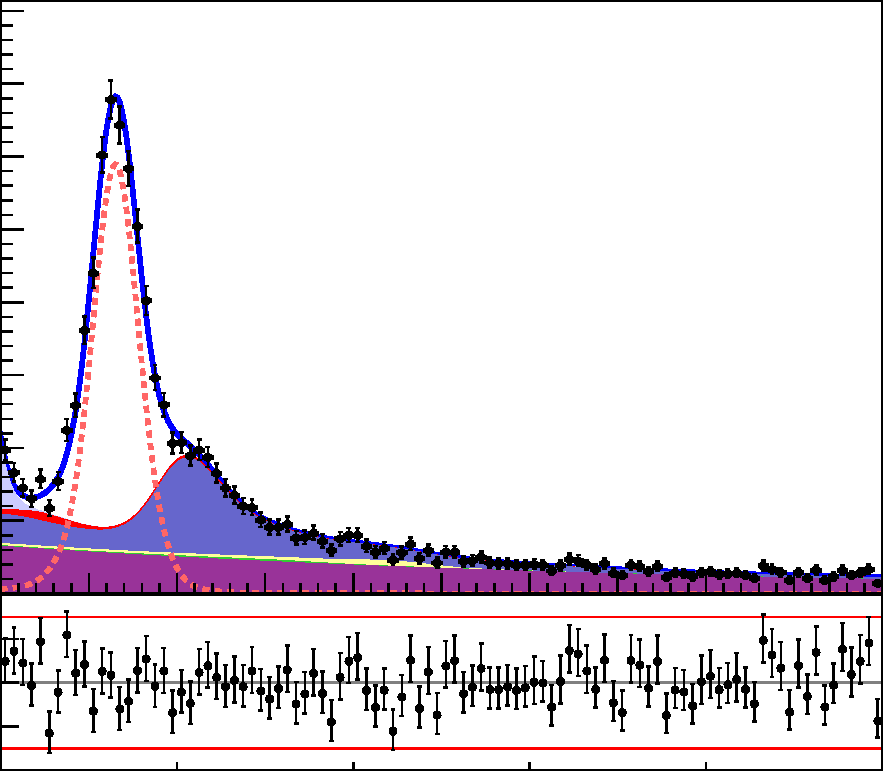
\includegraphics[width=0.675\textwidth]{appendices/mass_Bs2DsK_BeautyMass_both_all_2012_split}};
            \begin{scope}[x={(image.south east)},y={(image.north west)}]
                \foreach \x/\xtext in {5300, 5400, ..., 5800}
                {
                    \tikzmath{\xpos = (\x - 5300) / (5800 - 5300);}
                    \node at (\xpos, -0.040) {\(\xtext\)};
                }
                \foreach \y in {0, ..., 8}
                {
                    \tikzmath{\ypos = (\y / 8) * 0.749 + 0.207; \ytext = 100 * \y;}
                    \node[anchor=base east] at (0.012, \ypos) {\(\pgfmathprintnumber[fixed,precision=0,fixed zerofill=true,1000 sep={}]{\ytext}\)};
                }
                \foreach \p in {0, ..., 2}
                {
                    \tikzmath{\ypos = (\p / 2) * 0.120 + .055; \ptext = (\p - 1) * 2;}
                    \node[anchor=east] at (0.012, \ypos) {\(\scriptstyle\pgfmathprintnumber[fixed,precision=0,fixed zerofill=true]{\ptext}\)};
                }
                \node[anchor=east] at (1.0, -0.14) {\({m(\DsmpKpm)}~[\si{\MeVcc}]\)};
                \node[rotate=90,anchor=east,inner xsep=0pt,outer xsep=0pt] at (-0.20, 1.0) {\({\text{Candidates}/(\SI{5.0}{\MeVcc})}\)};
                \node[anchor=west] at (0.26, 0.92) {\large\lhcb};
            \end{scope}
        \end{tikzpicture}
        \caption{\DsmpKpm~invariant mass fit for the data taken at~\({\sqs = \SI{8}{\TeV}}\).}
    \end{subfigure}
    \\
    \begin{subfigure}{.48\textwidth} \centerfloat
        \begin{tikzpicture}
            \node[anchor=south west,inner sep=0] (image) at (0,0) {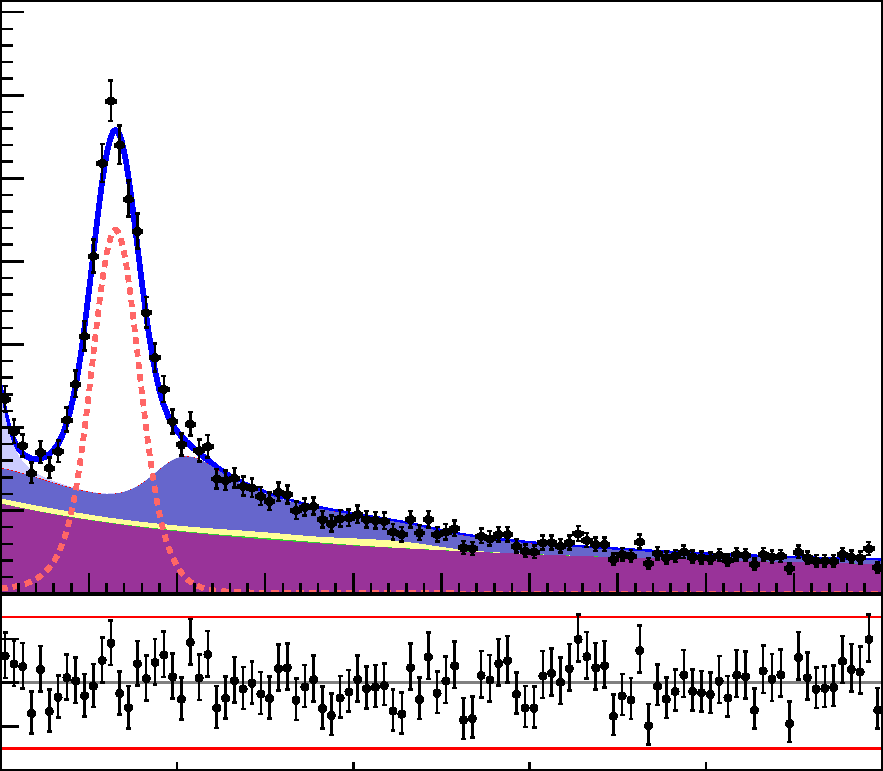
\includegraphics[width=0.675\textwidth]{appendices/mass_Bs2DsK_BeautyMass_both_all_run1_BDTG1}};
            \begin{scope}[x={(image.south east)},y={(image.north west)}]
                \foreach \x/\xtext in {5300, 5400, ..., 5800}
                {
                    \tikzmath{\xpos = (\x - 5300) / (5800 - 5300);}
                    \node at (\xpos, -0.040) {\(\xtext\)};
                }
                \foreach \y in {0, ..., 7}
                {
                    \tikzmath{\ypos = (\y / 7) * 0.749 + 0.207; \ytext = 100 * \y;}
                    \node[anchor=base east] at (0.012, \ypos) {\(\pgfmathprintnumber[fixed,precision=0,fixed zerofill=true,1000 sep={}]{\ytext}\)};
                }
                \foreach \p in {0, ..., 2}
                {
                    \tikzmath{\ypos = (\p / 2) * 0.120 + .055; \ptext = (\p - 1) * 2;}
                    \node[anchor=east] at (0.012, \ypos) {\(\scriptstyle\pgfmathprintnumber[fixed,precision=0,fixed zerofill=true]{\ptext}\)};
                }
                \node[anchor=east] at (1.0, -0.14) {\({m(\DsmpKpm)}~[\si{\MeVcc}]\)};
                \node[rotate=90,anchor=east,inner xsep=0pt,outer xsep=0pt] at (-0.20, 1.0) {\({\text{Candidates}/(\SI{5.0}{\MeVcc})}\)};
                \node[anchor=west] at (0.26, 0.92) {\large\lhcb};
            \end{scope}
        \end{tikzpicture}
        \caption{\DsmpKpm~invariant mass fit for the data taken with a low BDT~response.}
    \end{subfigure}
    \begin{subfigure}{.48\textwidth} \centerfloat
        \begin{tikzpicture}
            \node[anchor=south west,inner sep=0] (image) at (0,0) {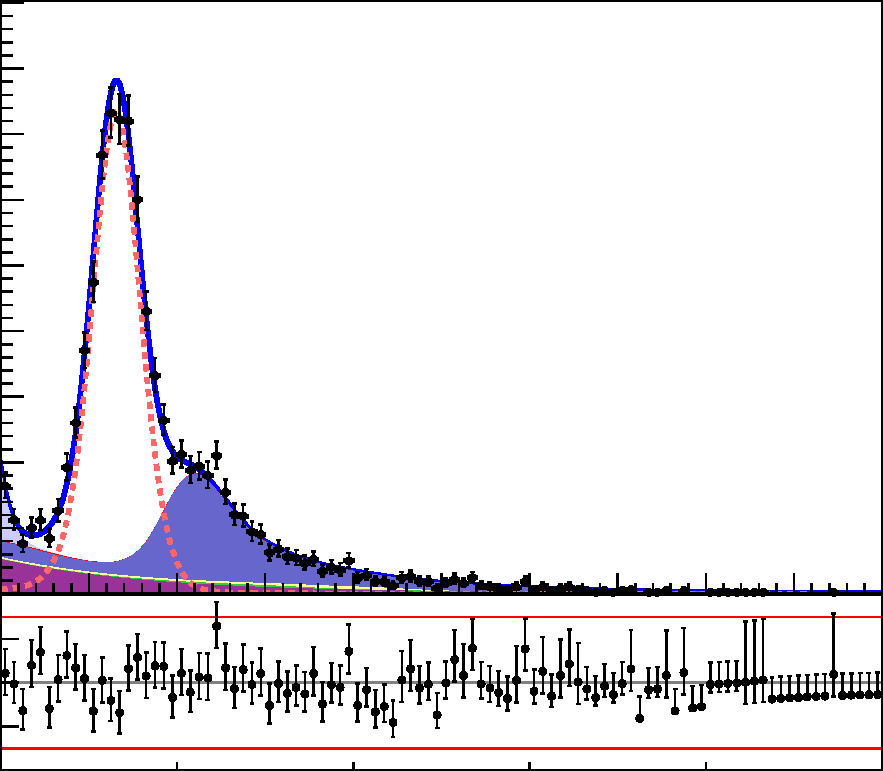
\includegraphics[width=0.675\textwidth]{appendices/mass_Bs2DsK_BeautyMass_both_all_run1_BDTG2}};
            \begin{scope}[x={(image.south east)},y={(image.north west)}]
                \foreach \x/\xtext in {5300, 5400, ..., 5800}
                {
                    \tikzmath{\xpos = (\x - 5300) / (5800 - 5300);}
                    \node at (\xpos, -0.040) {\(\xtext\)};
                }
                \foreach \y in {0, ..., 9}
                {
                    \tikzmath{\ypos = (\y / 9) * 0.760 + 0.207; \ytext = 50 * \y;}
                    \node[anchor=base east] at (0.012, \ypos) {\(\pgfmathprintnumber[fixed,precision=0,fixed zerofill=true,1000 sep={}]{\ytext}\)};
                }
                \foreach \p in {0, ..., 2}
                {
                    \tikzmath{\ypos = (\p / 2) * 0.120 + .055; \ptext = (\p - 1) * 2;}
                    \node[anchor=east] at (0.012, \ypos) {\(\scriptstyle\pgfmathprintnumber[fixed,precision=0,fixed zerofill=true]{\ptext}\)};
                }
                \node[anchor=east] at (1.0, -0.14) {\({m(\DsmpKpm)}~[\si{\MeVcc}]\)};
                \node[rotate=90,anchor=east,inner xsep=0pt,outer xsep=0pt] at (-0.20, 1.0) {\({\text{Candidates}/(\SI{5.0}{\MeVcc})}\)};
                \node[anchor=west] at (0.26, 0.92) {\large\lhcb};
            \end{scope}
        \end{tikzpicture}
        \caption{\DsmpKpm~invariant mass fit for the data taken with a high BDT~response.}
    \end{subfigure}

    \caption{
        Results of the split multivariate fits to \BsDsK~candidates, as described in \cref{sec:BsDsK_TD_MDFit_Validation}.}
\end{figure}

\chapter{Split decay-time fits}
\label{app:SplitTimeFits}

This \lcnamecref{app:SplitTimeFits} contains the figures of the decay-time fits to partial samples of \BsDsPi~candidates, introduced in \cref{sec:BsDsK_TD_CrossChecks}.
%
\begin{figure}[hp] \centerfloat
    \fontsize{8}{9.6}\selectfont
    \begin{subfigure}{.48\textwidth} \centerfloat
        \begin{tikzpicture}
            \node[anchor=south west,inner sep=0] (image) at (0,0) {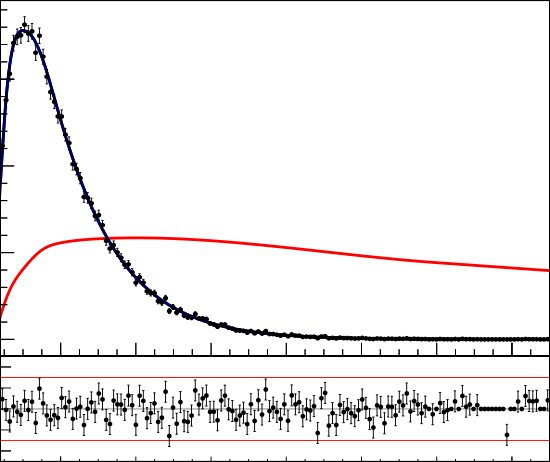
\includegraphics[width=0.675\textwidth]{appendices/time_Bs2DsPi_up}};
            \begin{scope}[x={(image.south east)},y={(image.north west)}]
                \foreach \x in {0, ..., 6}
                {
                    \tikzmath{\xpos = (\x / 6) * (0.931 - 0.111) + 0.111; \xtext = 2 * \x + 2;}
                    \node at (\xpos, -0.040) {\(\pgfmathprintnumber[fixed,precision=0,fixed zerofill=true]{\xtext}\)};
                }
                \foreach \y in {0, ..., 3}
                {
                    \tikzmath{\ypos = (\y / 3) * (0.831 - 0.265) + 0.265; \ytext = 500 * \y;}
                    \node[anchor=east] at (0.012, \ypos) {\(\pgfmathprintnumber[fixed,precision=0,fixed zerofill=true,1000 sep={}]{\ytext}\)};
                }
                \foreach \p in {0, ..., 4}
                {
                    \tikzmath{\ypos = (\p / 4) * (0.206 - 0.027) + 0.027; \ptext = (\p - 2) * 2;}
                    \node[anchor=east] at (0.012, \ypos) {\(\scriptstyle\pgfmathprintnumber[fixed,precision=0,fixed zerofill=true]{\ptext}\)};
                }
                \node[anchor=east] at (1.0, -0.14) {Decay time~\([\si{\ps}]\)};
                \node[rotate=90,anchor=east,inner xsep=0pt,outer xsep=0pt] at (-0.20, 1.0) {\({\text{Candidates}/(\SI{0.10}{\ps})}\)};
                \node[anchor=west] at (0.54, 0.89) {\large\lhcb};
            \end{scope}
        \end{tikzpicture}
        \caption{\DsmpPipm~invariant mass fit for the data taken with the \lhcb~magnet polarity up.}
    \end{subfigure}
    \begin{subfigure}{.48\textwidth} \centerfloat
        \begin{tikzpicture}
            \node[anchor=south west,inner sep=0] (image) at (0,0) {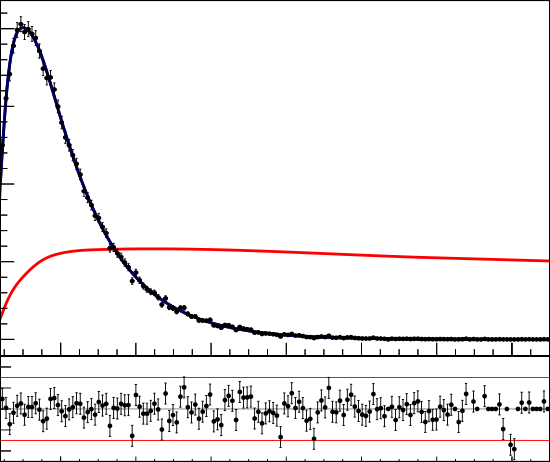
\includegraphics[width=0.675\textwidth]{appendices/time_Bs2DsPi_down}};
            \begin{scope}[x={(image.south east)},y={(image.north west)}]
                \foreach \x in {0, ..., 6}
                {
                    \tikzmath{\xpos = (\x / 6) * (0.931 - 0.111) + 0.111; \xtext = 2 * \x + 2;}
                    \node at (\xpos, -0.040) {\(\pgfmathprintnumber[fixed,precision=0,fixed zerofill=true]{\xtext}\)};
                }
                \foreach \y in {0, ..., 4}
                {
                    \tikzmath{\ypos = (\y / 4) * (0.937 - 0.265) + 0.265; \ytext = 500 * \y;}
                    \node[anchor=east] at (0.012, \ypos) {\(\pgfmathprintnumber[fixed,precision=0,fixed zerofill=true,1000 sep={}]{\ytext}\)};
                }
                \foreach \p in {0, ..., 4}
                {
                    \tikzmath{\ypos = (\p / 4) * (0.206 - 0.027) + 0.027; \ptext = (\p - 2) * 2;}
                    \node[anchor=east] at (0.012, \ypos) {\(\scriptstyle\pgfmathprintnumber[fixed,precision=0,fixed zerofill=true]{\ptext}\)};
                }
                \node[anchor=east] at (1.0, -0.14) {Decay time~\([\si{\ps}]\)};
                \node[rotate=90,anchor=east,inner xsep=0pt,outer xsep=0pt] at (-0.20, 1.0) {\({\text{Candidates}/(\SI{0.10}{\ps})}\)};
                \node[anchor=west] at (0.54, 0.89) {\large\lhcb};
            \end{scope}
        \end{tikzpicture}
        \caption{\DsmpPipm~invariant mass fit for the data taken with the \lhcb~magnet polarity down.}
    \end{subfigure}
    \\
    \begin{subfigure}{.48\textwidth} \centerfloat
        \begin{tikzpicture}
            \node[anchor=south west,inner sep=0] (image) at (0,0) {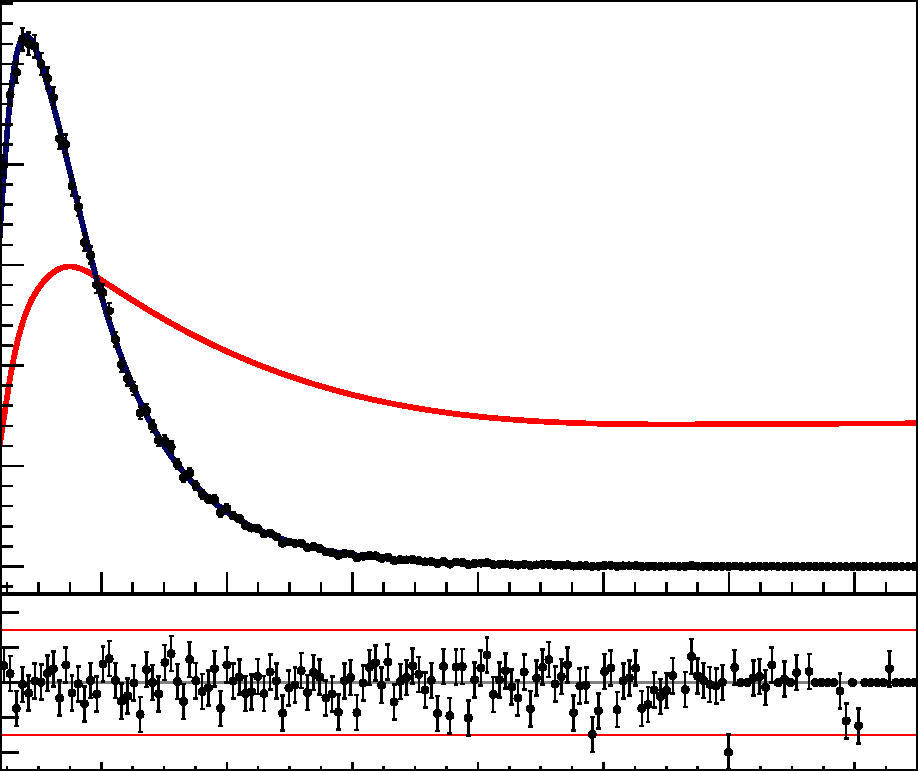
\includegraphics[width=0.675\textwidth]{appendices/time_Bs2DsPi_BDTG1}};
            \begin{scope}[x={(image.south east)},y={(image.north west)}]
                \foreach \x in {0, ..., 6}
                {
                    \tikzmath{\xpos = (\x / 6) * (0.931 - 0.111) + 0.111; \xtext = 2 * \x + 2;}
                    \node at (\xpos, -0.040) {\(\pgfmathprintnumber[fixed,precision=0,fixed zerofill=true]{\xtext}\)};
                }
                \foreach \y in {0, ..., 5}
                {
                    \tikzmath{\ypos = (\y / 5) * (0.916 - 0.265) + 0.265; \ytext = 500 * \y;}
                    \node[anchor=east] at (0.012, \ypos) {\(\pgfmathprintnumber[fixed,precision=0,fixed zerofill=true,1000 sep={}]{\ytext}\)};
                }
                \foreach \p in {0, ..., 4}
                {
                    \tikzmath{\ypos = (\p / 4) * (0.206 - 0.027) + 0.027; \ptext = (\p - 2) * 2;}
                    \node[anchor=east] at (0.012, \ypos) {\(\scriptstyle\pgfmathprintnumber[fixed,precision=0,fixed zerofill=true]{\ptext}\)};
                }
                \node[anchor=east] at (1.0, -0.14) {Decay time~\([\si{\ps}]\)};
                \node[rotate=90,anchor=east,inner xsep=0pt,outer xsep=0pt] at (-0.20, 1.0) {\({\text{Candidates}/(\SI{0.10}{\ps})}\)};
                \node[anchor=west] at (0.54, 0.89) {\large\lhcb};
            \end{scope}
        \end{tikzpicture}
        \caption{\DsmpPipm~invariant mass fit for the data taken with a low BDT~response.}
    \end{subfigure}
    \begin{subfigure}{.48\textwidth} \centerfloat
        \begin{tikzpicture}
            \node[anchor=south west,inner sep=0] (image) at (0,0) {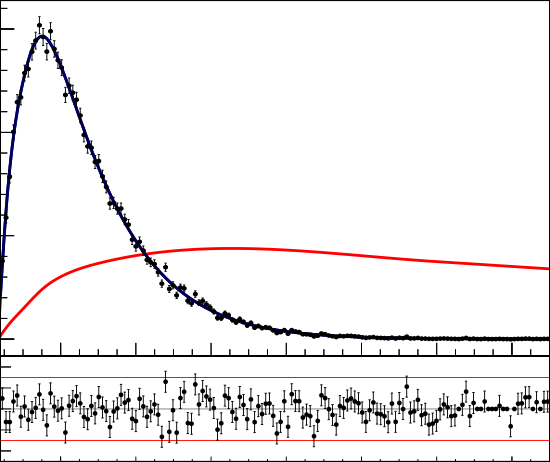
\includegraphics[width=0.675\textwidth]{appendices/time_Bs2DsPi_BDTG2}};
            \begin{scope}[x={(image.south east)},y={(image.north west)}]
                \foreach \x in {0, ..., 6}
                {
                    \tikzmath{\xpos = (\x / 6) * (0.931 - 0.111) + 0.111; \xtext = 2 * \x + 2;}
                    \node at (\xpos, -0.040) {\(\pgfmathprintnumber[fixed,precision=0,fixed zerofill=true]{\xtext}\)};
                }
                \foreach \y in {0, ..., 3}
                {
                    \tikzmath{\ypos = (\y / 3) * (0.936 - 0.265) + 0.265; \ytext = 500 * \y;}
                    \node[anchor=east] at (0.012, \ypos) {\(\pgfmathprintnumber[fixed,precision=0,fixed zerofill=true,1000 sep={}]{\ytext}\)};
                }
                \foreach \p in {0, ..., 4}
                {
                    \tikzmath{\ypos = (\p / 4) * (0.206 - 0.027) + 0.027; \ptext = (\p - 2) * 2;}
                    \node[anchor=east] at (0.012, \ypos) {\(\scriptstyle\pgfmathprintnumber[fixed,precision=0,fixed zerofill=true]{\ptext}\)};
                }
                \node[anchor=east] at (1.0, -0.14) {Decay time~\([\si{\ps}]\)};
                \node[rotate=90,anchor=east,inner xsep=0pt,outer xsep=0pt] at (-0.20, 1.0) {\({\text{Candidates}/(\SI{0.10}{\ps})}\)};
                \node[anchor=west] at (0.54, 0.89) {\large\lhcb};
            \end{scope}
        \end{tikzpicture}
        \caption{\DsmpPipm~invariant mass fit for the data taken with a high BDT~response.}
    \end{subfigure}
    \\
    \begin{subfigure}{.48\textwidth} \centerfloat
        \begin{tikzpicture}
            \node[anchor=south west,inner sep=0] (image) at (0,0) {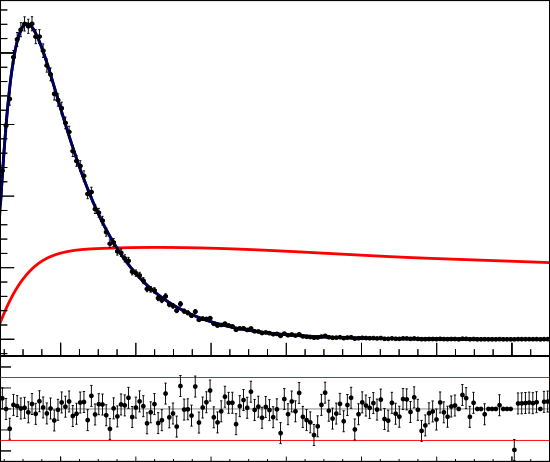
\includegraphics[width=0.675\textwidth]{appendices/time_Bs2DsPi_BsP1}};
            \begin{scope}[x={(image.south east)},y={(image.north west)}]
                \foreach \x in {0, ..., 6}
                {
                    \tikzmath{\xpos = (\x / 6) * (0.931 - 0.111) + 0.111; \xtext = 2 * \x + 2;}
                    \node at (\xpos, -0.040) {\(\pgfmathprintnumber[fixed,precision=0,fixed zerofill=true]{\xtext}\)};
                }
                \foreach \y in {0, ..., 4}
                {
                    \tikzmath{\ypos = (\y / 4) * (0.885 - 0.265) + 0.265; \ytext = 500 * \y;}
                    \node[anchor=east] at (0.012, \ypos) {\(\pgfmathprintnumber[fixed,precision=0,fixed zerofill=true,1000 sep={}]{\ytext}\)};
                }
                \foreach \p in {0, ..., 4}
                {
                    \tikzmath{\ypos = (\p / 4) * (0.206 - 0.027) + 0.027; \ptext = (\p - 2) * 2;}
                    \node[anchor=east] at (0.012, \ypos) {\(\scriptstyle\pgfmathprintnumber[fixed,precision=0,fixed zerofill=true]{\ptext}\)};
                }
                \node[anchor=east] at (1.0, -0.14) {Decay time~\([\si{\ps}]\)};
                \node[rotate=90,anchor=east,inner xsep=0pt,outer xsep=0pt] at (-0.20, 1.0) {\({\text{Candidates}/(\SI{0.10}{\ps})}\)};
                \node[anchor=west] at (0.54, 0.89) {\large\lhcb};
            \end{scope}
        \end{tikzpicture}
        \caption{\DsmpPipm~invariant mass fit for the data with a \Bs~candidate momentum \({< \SI{120}{\GeVcc}}\).}
    \end{subfigure}
    \begin{subfigure}{.48\textwidth} \centerfloat
        \begin{tikzpicture}
            \node[anchor=south west,inner sep=0] (image) at (0,0) {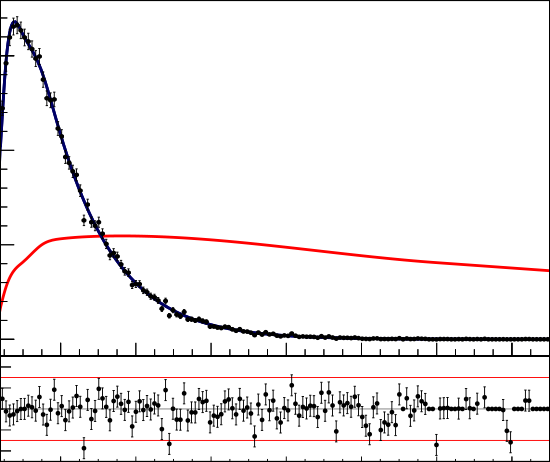
\includegraphics[width=0.675\textwidth]{appendices/time_Bs2DsPi_BsP2}};
            \begin{scope}[x={(image.south east)},y={(image.north west)}]
                \foreach \x in {0, ..., 6}
                {
                    \tikzmath{\xpos = (\x / 6) * (0.931 - 0.111) + 0.111; \xtext = 2 * \x + 2;}
                    \node at (\xpos, -0.040) {\(\pgfmathprintnumber[fixed,precision=0,fixed zerofill=true]{\xtext}\)};
                }
                \foreach \y in {0, ..., 3}
                {
                    \tikzmath{\ypos = (\y / 3) * (0.878 - 0.265) + 0.265; \ytext = 500 * \y;}
                    \node[anchor=east] at (0.012, \ypos) {\(\pgfmathprintnumber[fixed,precision=0,fixed zerofill=true,1000 sep={}]{\ytext}\)};
                }
                \foreach \p in {0, ..., 4}
                {
                    \tikzmath{\ypos = (\p / 4) * (0.206 - 0.027) + 0.027; \ptext = (\p - 2) * 2;}
                    \node[anchor=east] at (0.012, \ypos) {\(\scriptstyle\pgfmathprintnumber[fixed,precision=0,fixed zerofill=true]{\ptext}\)};
                }
                \node[anchor=east] at (1.0, -0.14) {Decay time~\([\si{\ps}]\)};
                \node[rotate=90,anchor=east,inner xsep=0pt,outer xsep=0pt] at (-0.20, 1.0) {\({\text{Candidates}/(\SI{0.10}{\ps})}\)};
                \node[anchor=west] at (0.54, 0.89) {\large\lhcb};
            \end{scope}
        \end{tikzpicture}
        \caption{\DsmpPipm~invariant mass fit for the data with a \Bs~candidate momentum \({> \SI{120}{\GeVcc}}\).}
    \end{subfigure}

    \caption{
        Results of the split decay-time fits to \BsDsPi~candidates, as described in \cref{sec:BsDsK_TD_CrossChecks}.}
\end{figure}
